\documentclass[12pt,twoside]{article}
\usepackage{amsmath, amssymb}
\usepackage{amsmath}
\usepackage[active]{srcltx}
\usepackage{amssymb}
\usepackage{amscd}
\usepackage{makeidx}
\usepackage{amsthm}
\usepackage{algpseudocode}
\usepackage{algorithm}
\usepackage{listings}
\usepackage{fancyhdr}
\usepackage{graphics}
%----------------------------------------------------------------------------------------------
\usepackage{amsmath, amssymb}
\usepackage{amsmath}
\usepackage[active]{srcltx}
\usepackage{amssymb}
\usepackage{amscd}
\usepackage{makeidx}
\usepackage[dvips]{graphicx}

\renewcommand{\baselinestretch}{1}
\setcounter{page}{1}
\setlength{\textheight}{21.6cm}
\setlength{\textwidth}{14cm}
\setlength{\oddsidemargin}{1cm}
\setlength{\evensidemargin}{1cm}
\pagestyle{myheadings}
\thispagestyle{empty}
\newtheorem{defi}{Definición}
\newtheorem{algoritmo}{Algoritmo}
\markboth{\small{Practica 5. Martínez López Sebastian, Ramírez Resendiz Luis Roque.}}{\small{.}}
\date{}
\begin{document}

\begin{figure}[h]
\vspace{-3cm} \hspace{-2cm} \setlength{\unitlength}{1mm}
\begin{picture}(15,25)(-10,0)

\includegraphics[width=16cm, height=4cm]{TITULO.JPG}
\end{picture}
\end{figure}


\vspace{0cm}

\centerline{\bf Análisis de Algoritmos, Sem: 2023-1, 3CV11, Práctica 6, Fecha: 28  Diciembre 2022}

\centerline{}

%\centerline{}


\begin{center}
\Large{\textsc{Práctica 6: Programación Dinámica}}
\end{center}
\centerline{}
\centerline{\bf {Martinez Lopez Sebastian, Ramirez Resendiz Luis Roque}} 
\centerline{}
\centerline{$sebastian.martinez.lopez98@gmail.com$, $luis\_roque\_ramirez@hotmail.com$}


\bigskip

\textbf{Resumen:} Se realizará el algoritmo de la Subsecuencia Común mas larga el cual comparara dos archivos de texto haciendo uso Programación Dinámica
\\
\\

{\bf Palabras Clave:} \textbf{Python, Arreglos, Recursividad, Programación Dinámica, Optimalidad, Subseciencia Común mas Larga, Archivos de texto}.
\newpage

\section{Introducci\'on}
El uso de los algoritmos tiene una importancia fundamental al momento de desarrollar diversos aplicativos, permitiéndo optimizar tareas hasta alcanzar que se realicen en el menor tiempo posible, consumiendo a su vez, la menor cantidad de recursos posibles.
\\
\\
Se sabe que cualquier algoritmos es nada mas y nada menos que la transformación de una tarea a una serie de instrucciones finitas y  precisas para que el computador pueda ejecutarlas y que se encuentran presentes en la vida cotidiana, como lo es cuando realizamos alguna receta de cocina, alguna actividad de limpieza como tender la cama entre otros.
Es decir un algoritmo es como un instructivo.
\\
\\
 Por eso, el objetivo principal de esta practica es poder analizar los algoritmos propuestos bajo el estudio de sus complejidades, que pueden ser la espacial S(n), refiriéndose a la cantidad de recursos de memoria, y la complejidad temporal f(n) en la cual nos enfocamos.
\\
\\
 A su vez, se enfoca en ver los datos estadísticos y las diferentes gráficas obtenidas de los mismos en los campos del tiempo de ejecución de los algoritmos propuestos, para a su vez determinar el análisis a posteriori y con esto poder llegar a una conclusión lo mas clara y precisa posible. 
\\
\\
Con la implementación de los dos algoritmos de programación dinámica y la subsecucia común mas larga, se garantiza el encontrar una solución optima, a lo cual se enfoca de manera principal en la optimización de los problemas, lo cual en la actualidad es muy complicado, esto se puede comprender con mayor facilidad con los ejemplos y con la comprensión de los algoritmos.
\\
\newpage



\section{Conceptos B\'asicos}
\begin{defi}[Algoritmo]
Acorde a la RAE, se puede definir la palabra algoritmo como "Conjunto ordenado y finito de operaciones que permite hallar la solución de un problema."
Sin embargo se puede complementar dicha informaci\'on tomando en cuenta las partes claves de un algoritmo.
Concluyendo así, en otras palabras que un algoritmo es un conjunto de pasos para resolver algo.
El algoritmo debe contemplar los siguientes puntos para que pueda ser considerado un algoritmo:
\begin{itemize}
\item Preciso: Un algoritmo debe ser claro y conciso para la tarea a realizar.
\item Finito: Un algoritmo no puede ser ejecutado infinitamente.
\item Definido: EL algoritmo debe tener un punto de finalización.
\end{itemize} 
Dentro del reporte, manejaremos a los algoritmos en su forma de pseudocodigo, como se puede apreciar en la figura 1(Figure 1: Diagrama de flujo de un algoritmo).
\begin{figure}[h!]
\centering
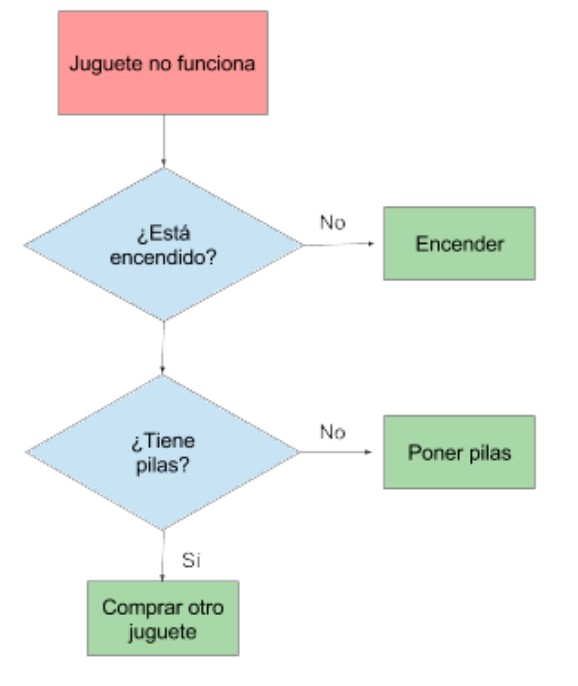
\includegraphics[scale=0.5]{algoritmo.jpg}
\caption{Diagrama de flujo de un algoritmo.}
\label{fig:universe}
\end{figure}

\end{defi}

\clearpage
\begin{defi}[Análisis a priori]
Acorde a la RAE, se puede definir la oraci\'on "a priori" c
omo  "‘por lo que precede’. En el ámbito de la filosofía, se emplea para referirse al conocimiento deductivo, esto es, al que se adquiere independientemente de la experiencia, yendo de las causas a los efectos y de lo universal a lo particular".
\\
En el analisis de algoritmos, se puede connotar que el analisis a priori sera aquel, el cual nos permita determinar la complejidad del mismo acorde a una notación, como lo pueden ser: Big O, $\Omega$, $\theta$.
\\
Para analizar dichos algoritmos es importante entender como funcionan los ordenes de complejidad dentro de los algoritmos, los cuales, podemos identificar en la siguiente tabla (Tabla 1: Orden de complejidad)
\\
\begin{table}[h!]
    \centering
    \begin{tabular}{|N|C|}
    \hline
        Orden & Nombre \\
    \hline
        O(1) & Constante \\
    \hline
        O($\log$ n) & Logarítmica \\
    \hline
        O(n) & lineal\\
    \hline
        O(n $\log$ n) & Casi lineal \\
    \hline
        O(n^{2}) & Cuadratica\\
    \hline
        O(n^{3}) & Cubica\\
    \hline
        O(a^{n}) & Exponencial\\
    \hline
    \end{tabular}
    \caption{Orden de complejidad}
    \label{tab:my_label}
\end{table}
\\
Asi mismo, se puede observar en la grafica siguiente, como se comportan cada uno de los ordenes de complejidad con relacion a su tasa de crecimiento,de donde el eje de las 'y' equivale al tiempo de ejecucion del algoritmo y en eje de las 'x' el contador, el cual idicara el orden de complejidad del algoritmo y a su vez sera delimitado por las cotas superior e inferior asintoticas, como se muestra en la siguiente figura (Figura 1: Tasa de crecimiento)

\begin{figure}[h!]
\centering
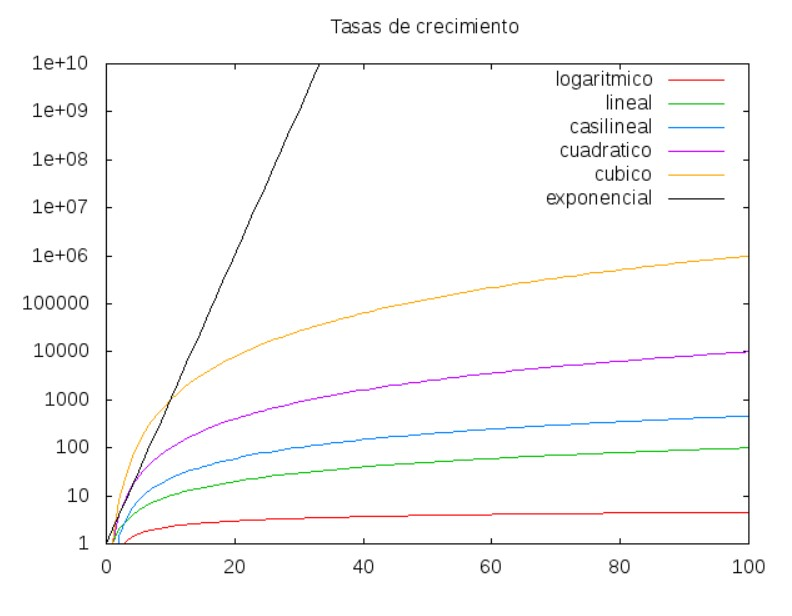
\includegraphics[scale=0.35]{orden de complejidad.jpg}
\caption{Tasa de crecimiento.}
\label{fig:tasa}
\end{figure}

\end{defi}
\clearpage
\\

\begin{defi}[Análisis a posteriori]
Acorde a la RAE, se define la oraci\'on "a posteriori" como  ‘por lo que viene después’. En el ámbito de la filosofía, se emplea para referirse al conocimiento inductivo, esto es, al que se adquiere a partir de la experiencia, ascendiendo de los efectos a las causas.
Así mismo, se connota que el an\'alisis a posteriori se recoge estadísticas de tiempo y espacio consumidas por el algoritmo mientras se ejecuta. 

\end{defi}
\begin{defi}[Notaci\'on O]
Es una herramienta que permite determinar la complejidad de un algoritmo determinando su rendimiento en cuanto a recursos y tiempo de ejecución, en pocas palabras identifica el peor caso donde el algoritmo llegue a su punto mas alto de exigencia.
\\
\\
Así mismo se acota de manera asintótica el crecimiento de un tiempo de ejecución a que este, dentro de factores constante por arriba y por abajo.
\\
\\
En la siguiente figura(Figura 3: Definicion Big O) se puede apreciar la cota superior asintotica, la cual esta resaltada en color azul. 
\begin{figure}[h!]
\centering
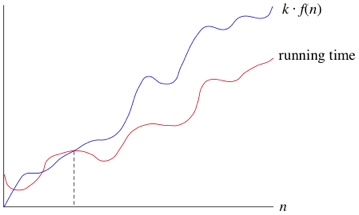
\includegraphics[scale=1.5]{big o.png}
\caption{Definici\'on Big O}
\label{fig:universe}
\end{figure}
\end{defi}
\clearpage
\begin{defi}[Notaci\'on $\Omega$]
Se usa la notación $\Omega$ para representar el limite asintótico inferior del tiempo de una funci\'on, esto quiere decir que, al contrario de la Notaci\'on O, se utiliza para calcularla complejidad de un algoritmo en su mejor caso.
\\
\\
En la siguiente grafica se puede apreciar lo que se denota como cota inferir asintotica, la cual esta resaltada en color azul.
\begin{figure}[h!]
\centering
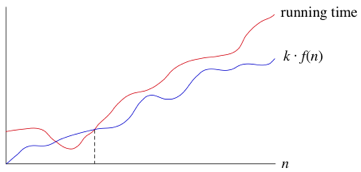
\includegraphics[scale=1.5]{big omega.png}
\caption{Definici\'on $\Omega$}
\label{fig:universe}
\end{figure}
\end{defi}

\begin{defi}[Notaci\'on $\Theta$]
Esta notaci\'on encierra a la funci\'on con un limite superior y un limite inferior. Se puede decir que se tiene una cota asintoticamente ajustada, esto por lo mencionado anteriormente ya que se ajusto el tiempo de ejecuci\'on (funci\'on) dentro del rango de una constante hacia arriba y hacia abajo. Esta notaci\'on se usa para calcular la complejidad de un algoritmo que no tiene mejor ni peor caso
\\
\\
En esta grafica se aprecia con mayor claridad ambas cotas, tanto la superior como la inferior, las cuales estan resaltadas en color azul. 
\begin{figure}[h!]
\centering
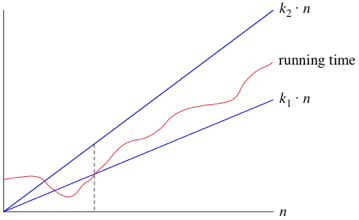
\includegraphics[scale=1.4]{big theta.png}
\caption{Definición $\Theta$}
\label{fig:universe}
\end{figure}
\end{defi}

\begin{defi}[Recursividad]
Acorde con la RAE, se define la "Recursividad" como "que se contiene a si mismo un numero indefinido de veces", es decir, en programacion se ve como la capacidad de una funcion de llamarse a si misma hasta cumplir una condicion de paro, es dedcir se repetira y llamara asi misma una 'n' cantidad de veces hasta poder resolver un determinado problema. 
\\
\\
\begin{figure}[h!]
\centering

\includegraphics[scale=.2]{recur.jpeg}
\caption{Definición Recursividad}
\label{fig:universe}
\end{figure}
\end{defi}

\begin{defi}[Optimalidad]
Cuando hablamos de optimizar nos referimos a buscar la mejor solución de entre muchas alternativas posibles. Dicho proceso de optimización puede ser visto como una secuencia de decisiones que nos proporcionan la solución correcta.
\\
\begin{figure}[h!]
\centering

\includegraphics[scale=.2]{opt.png}
\caption{Definición Optimalidad}
\label{fig:universe}
\end{figure}
\end{defi}
\newpage

\begin{defi}[Programación Dinámica]
es un método para reducir el tiempo de ejecución de un algoritmo mediante la utilización de subproblemas superpuestos y subestructuras óptimas.
\\
Una "subestructura óptima" significa que se pueden usar soluciones óptimas de subproblemas para encontrar la solución óptima del problema en su conjunto. Por ejemplo, el camino más corto entre dos vértices de un grafo se puede encontrar calculando primero el camino más corto al objetivo desde todos los vértices adyacentes al de partida, y después usando estas soluciones para elegir el mejor camino de todos ellos. En general, se pueden resolver problemas con subestructuras óptimas siguiendo estos tres pasos:
\\
\\
\begin{itemize}
\item Primer paso Dividir el problema en subproblemas más pequeños:
\\
\\
Descomponer el problema en sub-problemas del mismo tipo. Este paso involucra descomponer el problema original en pequeños sub-problemas. Cada sub-problema deberepresentar una parte del problema original. Por lo general, este paso emplea un enfoque recursivo para dividir el problema hasta que no es posible crear un sub-problema más.
\\
\item Segundo paso Resolver estos problemas de manera óptima usando este proceso de tres pasos recursivamente:
\\
\\
Resolver los sub-problemas recursivamente. Este paso recibe un gran conjunto de sub-problemas a ser resueltos. Generalmente a este nivel, los problemas se resuelven por sí solos.
\\
\item Tercer paso Usar estas soluciones óptimas para construir una solución óptima al problema original:
\\
\\
Combinar las respuestas apropiadamente. Cuando los sub-problemas son resueltos, esta fase los combina recursivamente hasta que estos formulan la solución al problema original. Este enfoque algorítmico trabaja recursivamente y los pasos de conquista y fusión trabajan tan a la par que parece un sólo paso.
\\
\end{itemize} 
\\
\end{defi}
\newpage

\begin{defi}[Subseciencia Común mas Larga]
El problema de subsecuencia común más larga, se trata de encontrar una subsecuencia más larga que es común en un conjunto de secuencias. Es diferente del problema de substring común más largo; a diferencia de los substrings, las subsecuencias no necesitan tener posiciones consecutivas en la secuencia original. El problema de LCS es uno de los problemas clásicos de las ciencias computacionales y es la base de programas que comparan datos como la utilidad diff, y ha tenido usos en bioinformática. También es usado ampliamente para los sistemas de control de revisión como Git para reconciliar múltiples cambios sobre archivos controlados de revisión.
\\
\begin{figure}[h!]
\centering
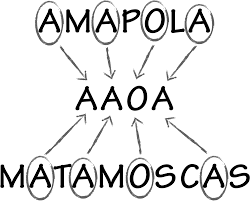
\includegraphics[scale=.5]{lcs.png}
\caption{Definición LCS}
\label{fig:universe}
\end{figure}
\end{defi}

\newpage

\begin{algoritmo}
Implementar un programa que permita comparar dos archivos de texto plano mediante Programación Dinámica haciendo uso del algoritmo de la Subsecuencia Común más Larga.
\lstinputlisting[language=Python]{Subsec.py}


\clearpage

\end{algoritmo}

 \section{Experimentaci\'on y Resultados}

\subsection{Algoritmo}
En el siguiente algoritmo se realizpo el analisis a priori en donde se observa la complehidad del mismo la cual es =(n*m), se debe a los recorridos con los ciclos for que realizan para comparar cada una de los textos, por lo tanto la complejidad es la antes mencionada. 

\\
Con la grafica se puede comprobar las complejidad previamente obtenida en los diversos analisis realid¿zados.
\\
\\
\subsubsection{}
\begin{figure}[h!]
\centering
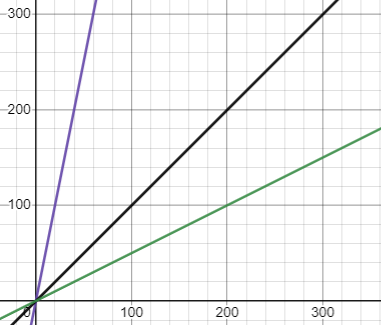
\includegraphics[scale=0.5]{graf.png}
\caption{Gráfica mostrando la complejidad}
\label{fig:universe}
\end{figure}

\clearpage


\section{Conclusiones}
Durante el desarrollo de esta practica la principal dificultad que se presento fue al momento de realiza la graficacion, mas precisamente al momento de definir las cotas superiores asintóticas y las cotas inferiores asintóticas, de igual manera al momento de calcular la diferente complejidad del algoritmo, ya que cada algoritmo cambia, porque en algunos de ellos se encuentran diferentes ciclos anidados como los ciclos while y ciclos if y ciclos for, una vez resuelto esto el resto fue mas sencillo, ahora bien, la interpretación que nosotros podemos darle a las gráficos.
\\
\\
Conclusión Martinez Lopez Sebastian:\\
Observamos que existen varios algoritmos para dar solución a un solo problema en especifico, con esto observamos que dependiendo de los diferentes requerimientos que nos hagan o requiera el programa es el algoritmo que podemos usar, ya que como paso en esta practica el algoritmo puede tener tres complejidades diferentes para diferentes casos y con esto podemos hacer que nuestro programa sea mas eficiente dependiendo del tipo de caso en el cual vaya a estar trabajando. 
\begin{figure}[h!]
\centering

\includegraphics[scale=0.2]{seb1.jpg}
\caption{}
\label{fig:universe}
\end{figure}
\\
Conclusión Ramirez Resendiz Luis Roque:\\
Podemos darnos cuenta que un solo algoritmo puede cambiar su complejidad dependiendo el caso en el que se encuentre y de esta manera nosotros podemos valorar y hacer un análisis a fondo sobre dicho algoritmo, permitiéndonos compararlo con otros algoritmos que resuelvan el mismo problema e implementando el algoritmo que mas nos convenga, obviamente basándonos en las necesidades o el para que requiramos el algoritmo. De igual manera s perceptible como en algunas ocaciones la recursividad o un algoritmo recursivo es mejor que un aloritmo iterativo, refiriendonos a su grado de complejidad. Ademas vemos que el concepto de optimización es un cocepto fuerte y debe utilizarse con mucho cuidado dado a que es muy complejo y dificil el poder dar una solución optima a algun problema.
\\
\\
De igual manera comprendemos que la programación dinámica es mucho mas complicada de llevar a acabop por la optimalidad, pero con ello seguramos que nuestra solución es una solución optima.
\begin{figure}[h!]
\centering

\includegraphics[scale=0.4]{luis1.jpg}
\caption{}
\label{fig:universe}
\end{figure}
\clearpage
\section{Bibliograf\'ia}
\\
Notación big O. (s/f). Pablocianes.com. Recuperado el 7 de septiembre de 2022, de https://pablocianes.com/notacion-big-o/
\\
\\
Notación Omega grande (Big-Ω). (s/f). Khan Academy. Recuperado el 7 de septiembre de 2022, de https://es.khanacademy.org/computing/computer-science/algorithms/asymptotic-notation/a/big-big-omega-notation
\\
\\
Notación θ grande (Big-θ). (s/f). Khan Academy. Recuperado el 7 de septiembre de 2022, de https://es.khanacademy.org/computing/computer-science/algorithms/asymptotic-notation/a/big-big-theta-notation
\\
\\
(S/f). Rae.es. Recuperado el 25 de octubre de 2022, de https://www.rae.es/dpd/a%20priori
\\
\\
(S/f-a). Rae.es. Recuperado el 25 de septiembre de 2022, de https://dle.rae.es/algoritmo
\\
\\
(S/f-b). Rae.es. Recuperado el 25 de septiembre de 2022, de https://www.rae.es/dpd/a%20posteriori
\\
\\
(S/f-c). Rae.es. Recuperado el 25 de septiembre de 2022, de https://www.rae.es/dpd/anterior
\\
\\
(S/f). Rae.es. Recuperado el 9 de noviembre de 2022, de https://dle.rae.es/recursivo
\\
\\
(S/f). Rae.es. Recuperado el 9 de noviembre de 2022, de https://dle.rae.es/iterativo
\\
\\

\medskip



\end{document}

